\graphicspath{{chapters/_resources/}}

\chapter{Chromosome domains and oncogene activation}

\section{Genome organization and transcription regulation}

\subsection{CTCF}
An enhancer can work at very high distance with respect to the gene of interest; this means that enhancers have the possibility to regulate many different promoters. How can enhancer activity be directed to a specific target?

\textbf{\emph{Insulator sequences}} prevent the propagation of enhancers signals along the chromatin fiber through their enhancer blocking function mediated by proteins. Insulator genes are usually found at a region densely distributed with genes. They can act in long distance, do not need specific direction and the sequences are recognized by proteins. The main insulator binding protein is a factor called CCCTC-binding factor (CTCF).

\textbf{CTCF} has a peculiar DBD with 11 zinc fingers; each of them can recognize a short consensus motif. In principle, it could recognize huge regions and be very flexible in recognition capabilities, as combinatorial use of its 11 ZF allows binding to 50bp target sites with high sequence variations. CTCF regulates transcription both positively and negatively and can operate as a transcription factor. At first, it was recognized as a repressive TF: it has the ability to shape the DNA molecules, not merely binding on a site distorting it, and to recruit co-factors.

CTCF is the main \emph{insulator-binding protein} in vertebrates. ChIP shows that CTCF binds thousands of sites in the human genome. We can find it mainly in intergenic regions and introns, as well as promoter regions. The consensus sequence recognized by CTCF is the same among cell lines.

CTCF is enriched at the H3K27me3 domain boundaries (CTCF barrier sites). A larger genomic region was analyzed in different cell lines. Almost no overlap was found in the CTCF barrier sites between CD4T cells and HeLa cells, suggesting that CTCF barriers are cell-type-specific. In some cells the site is at the boundary, in others not.

We know now that heterochromatic marks spread up to insulator sequences, which can be recognized by proteins and recruit directly or indirectly chromatin remodelling factors.

Main findings:

\begin{itemize}
\tightlist
\item
  CTCF can bind to the same locus in different cell types
\item
  CTCF binding can separate active and repressed chromatin, functioning as barrier to heterochromatin spreading
\item
  CTCF exerts its barrier ability in a cell type dependent manner
\end{itemize}

The function of CTCF appears to be regulated at least at two levels:

\begin{enumerate}
\def\labelenumi{\arabic{enumi}.}
\tightlist
\item
  binding of CTCF to the target sites
\item
  binding of interacting proteins, providing its functionality
\end{enumerate}

\hypertarget{cohesin-mediates-transcriptional-insulation-by-ccctc-binding-factor}{%
\subsection{Cohesin mediates transcriptional insulation by CCCTC-binding factor}\label{cohesin-mediates-transcriptional-insulation-by-ccctc-binding-factor}}

CTCF was found to interact with cohesins (composed of SMC3, SMC1, SCC1 and SCC3 subunits), which are essential to maintain sister chromatids connected from S phase to metaphase. Cohesins are loaded on chromosomes during G1, but their function is exerted later on. For achieving anaphase, the ring is cut by securins - regulated by APC.

\textbf{Cohesin} is expressed in differentiated postmitotic cells. We expect that replicating cells express cohesin, as it is heavily required during the cell cycle. Pulling down SMC3 in mouse brain we still observe a signal, it is probably linked to an additional function of the complex. During G2 we expect that cohesins are holding together sister chromatids, which instead are absent in G1; the binding site is the same, checked by ChIP-Seq $\rightarrow$ cohesin binds to the same sites independently of CTCF cohesion and cohesins share several binding sites (Figure \ref{fig:chip}).

\begin{figure}
\centering
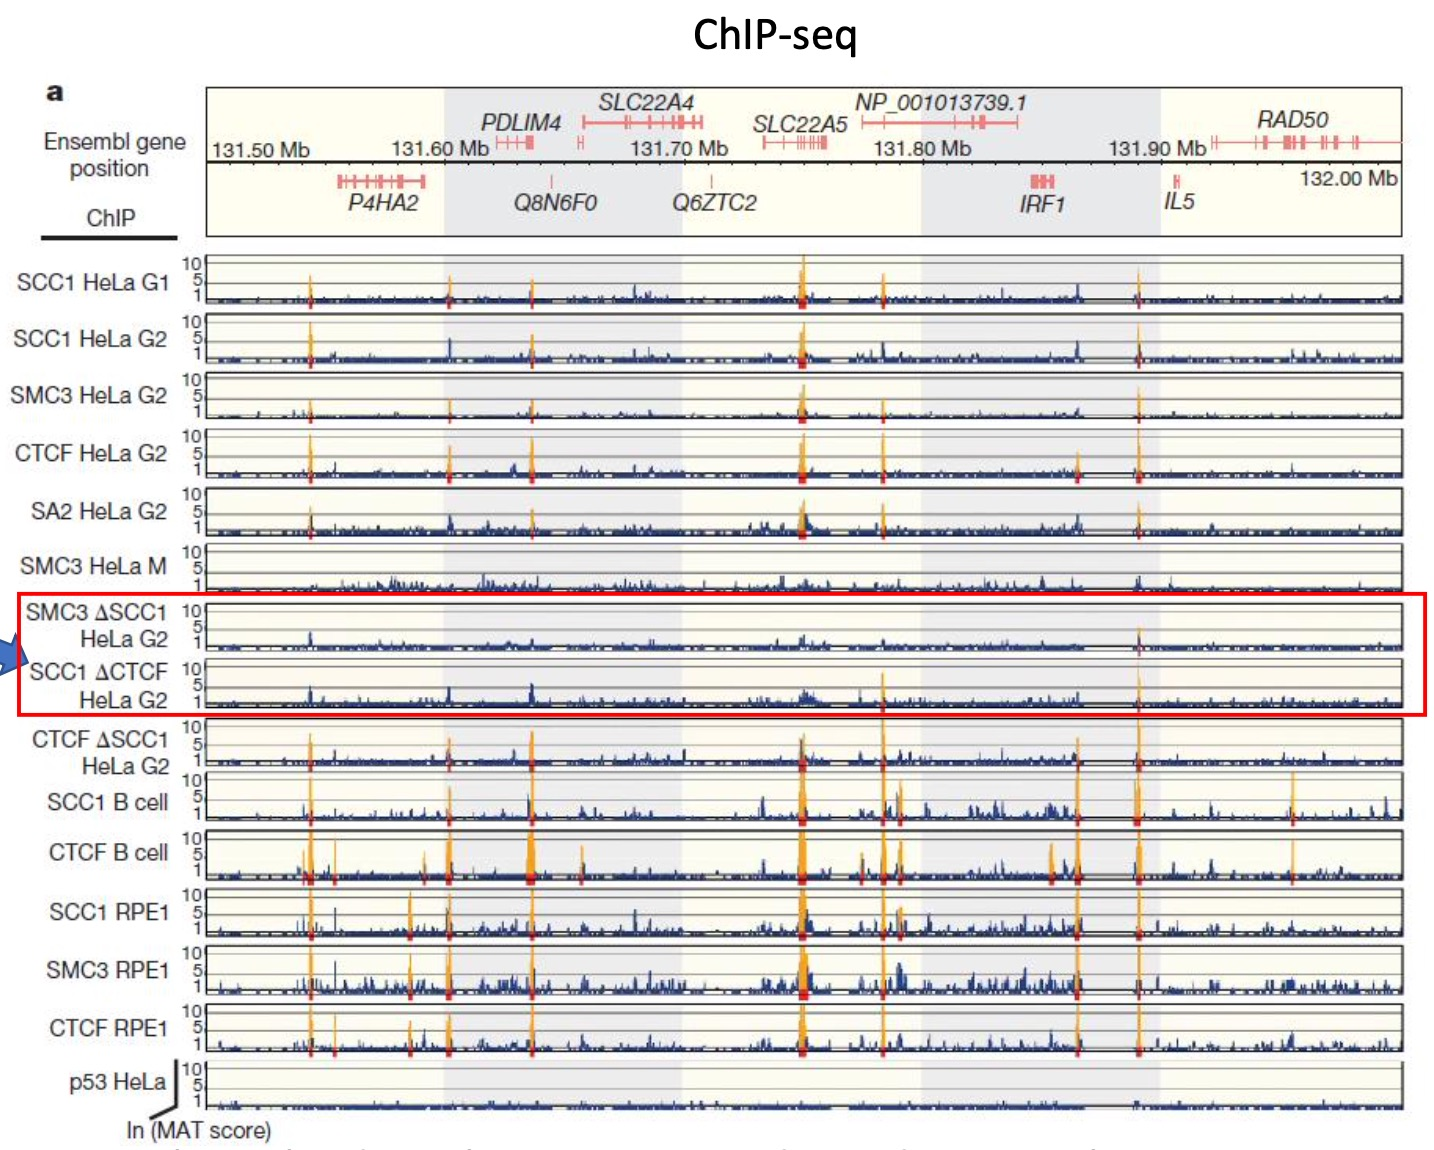
\includegraphics[width=0.5\textwidth]{../_resources/Screenshot_2022-10-14_at_19-51-43.png}
\caption{Yatskevich et al., Annu Rev Genet. 2019}
\label{fig:chip}
\end{figure}

By looking at CTCF KO the binding is lost, as well as SCC1 binding. Cohesin and CTCF co-occupy thousands of genomic binding sites and share the same consensus sequence. 

\emph{Does cohesion contribute to CTCF enhancer blocking function?}

Reporter assay with pIHLIE, which is known to be responsible for the insulator sequence (Figure \ref{fig:rep}). By removing CTCF, the luciferase activity increases. Nothing happens by impairing the sister chromatids' link through a drug, Sororin. The insulator function of H19 ICR requires CTCF binding as well as cohesin binding to DNA, but not the establishment of cohesion.

\begin{figure}
\centering
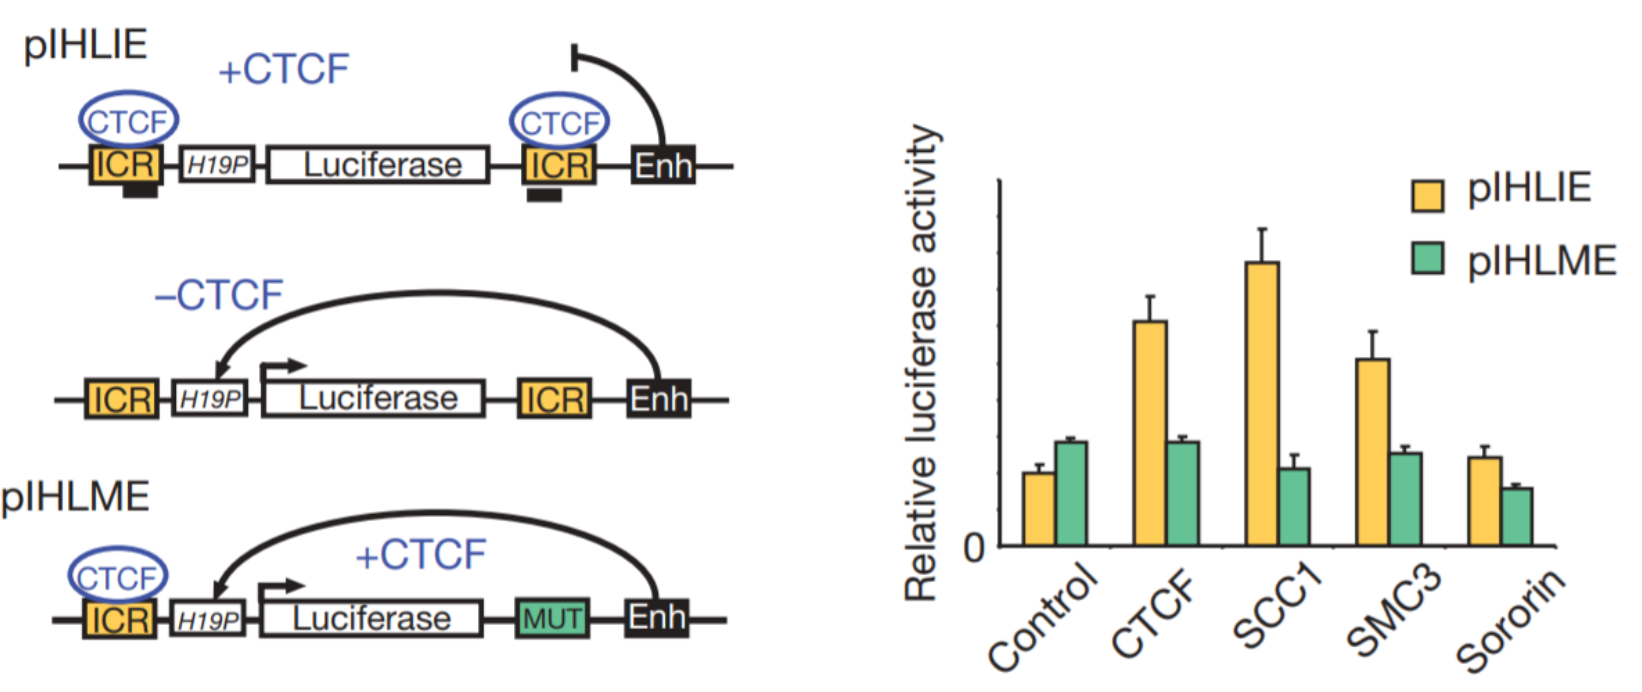
\includegraphics[width=0.8\textwidth]{../_resources/Screenshot_2022-10-14_at_19-50-44.png}
\caption{Wendt et al, Nature, 2008}
\label{fig:rep}
\end{figure}

Cohesin complexes co-localize with CTCF insulator protein and are required for it to block enhancer sequences (Figure \ref{fig:cohe}). CTCF can slide on DNA and stop when it reaches an already bound CTCF $\rightarrow$ functional to repress enhancer function (Figure \ref{fig:chrom}).

\begin{figure}[!htb]
   \begin{minipage}{0.48\textwidth}
     \centering
     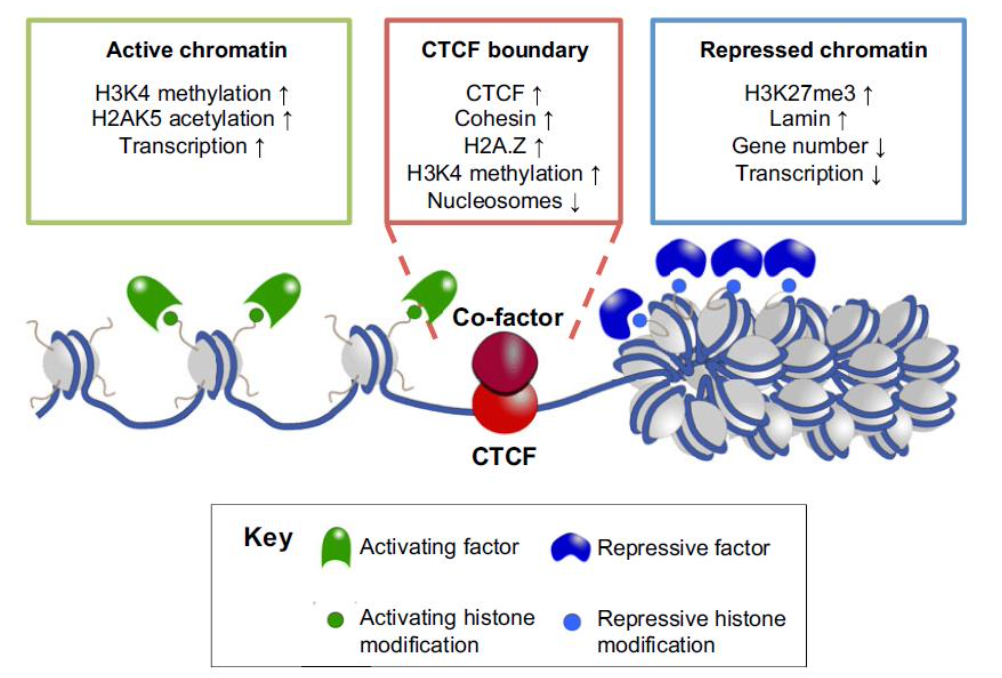
\includegraphics[width=0.6\textwidth]{../_resources/Screenshot_2022-10-14_at_12-11-11.png}
\caption{Herold \emph{et al., Development,} 2012}
\label{fig:chrom}
   \end{minipage}\hfill
   \begin{minipage}{0.48\textwidth}
     \centering
     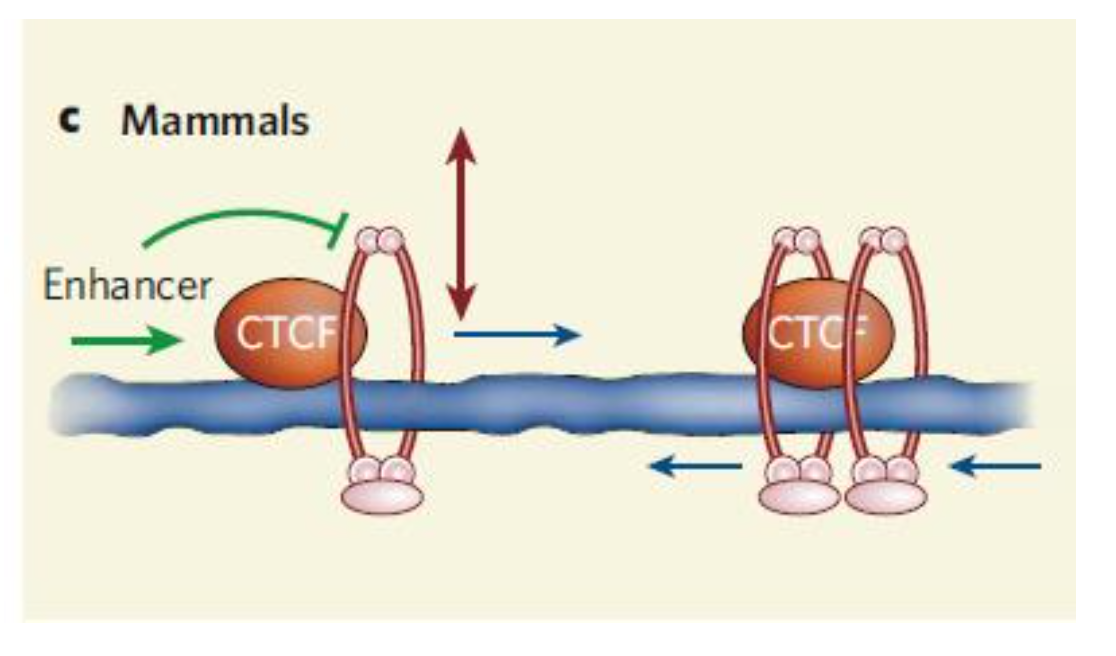
\includegraphics[width=0.5\textwidth]{../_resources/Screenshot_2022-10-14_at_12-10-46.png}
\caption{Parelho et al, Cell, 2008}
\label{fig:cohe}
   \end{minipage}
\end{figure}

\emph{Does cohesin have anything to do with transcription regulation?}
Upon CTCF insulator protein (orange) binding to its DNA consensus sequence, the cohesin ring may tether two DNA double strands (red--blue helices) by encircling them. Thus, \textbf{cohesion-CTCF complexes could shield genes from the effect of enhancer sequences}, regulating gene expression by impacting genome organization.

\subsection{CTCF and Cohesin in Genome Folding and Transcriptional Gene Regulation}

CTCF binding motifs tend to interact with each other forming a \emph{chromatin loop}. During interphase, DNA is not condensed as in a canonical chromosome, each chromosome forms territories with a hierarchical distribution of 3D folding. Different territories can overlap with each other, depending on the extent of histone modifications. We find compartments, territories and 3D folding of chromatin made by loops. Loops are possibly obtained thanks to the action of cohesins: in \textbf{\emph{loop extrusion}}, a cohesin can slide on DNA for circling 2 ds filaments, until it reaches CTCF is a specific direction. The directionality of CTCF DNA sequences at the loop boundaries indicates the presence of a ``tracking'' mode for DNA loop formation instead of a simple 3D diffusion.

\begin{figure}
\centering
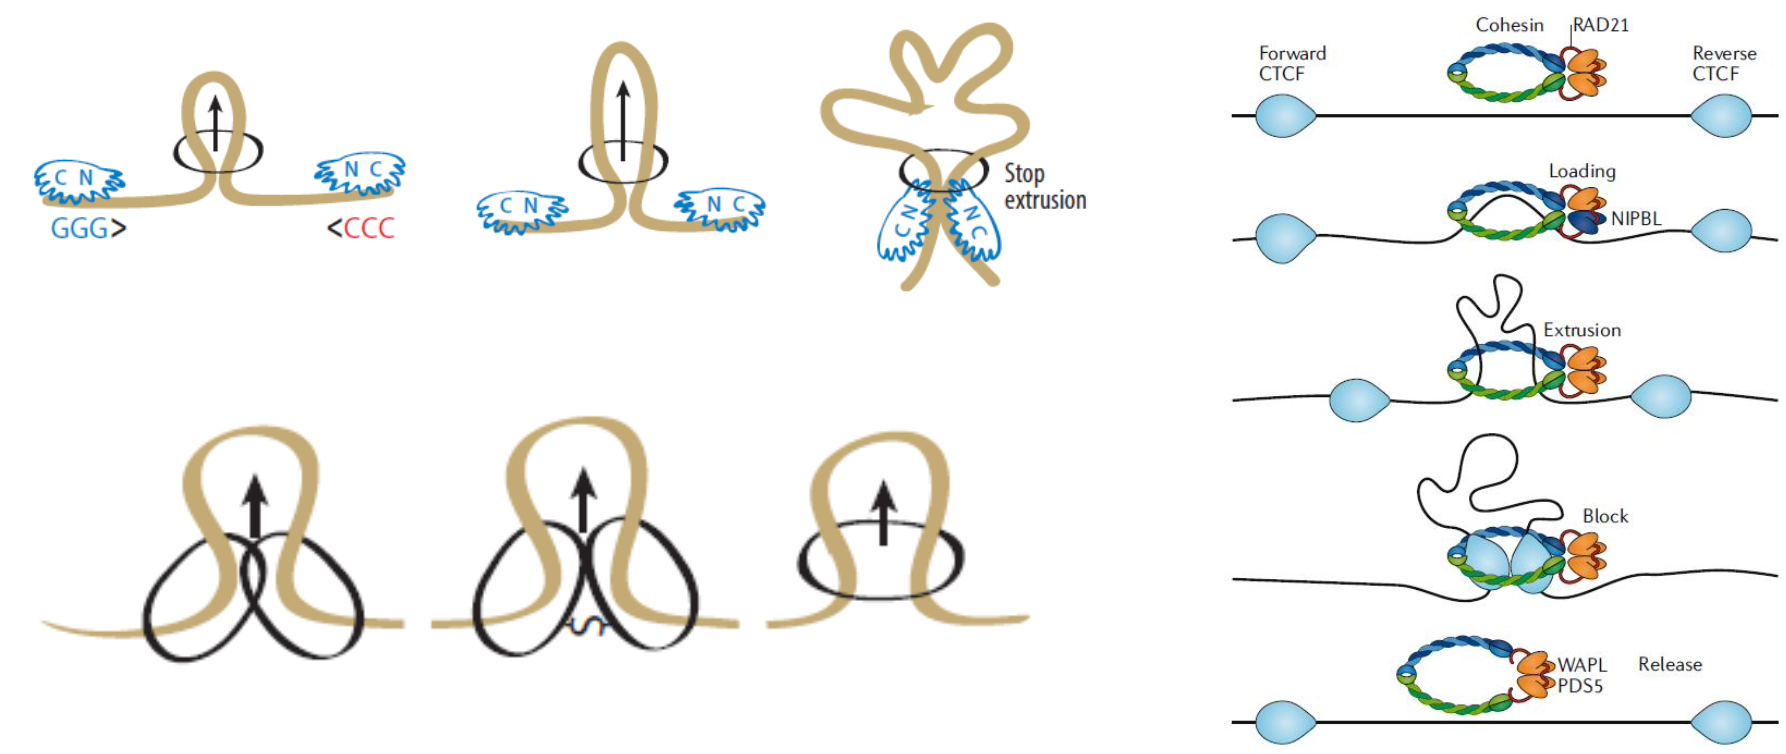
\includegraphics[width=0.6\textwidth]{../_resources/Screenshot_2022-10-14_at_19-52-56.png}
\caption{Merkenschlager and Nora, Ann Rev Gen Hum Genetics, 2016}
\end{figure}

The hierarchical model of chromatin organization impacts gene regulation:
\begin{itemize}
\tightlist
\item
  linear chromosome map-
\item
  local 3D folding: local folding brings convergent pairs of CTCF sites in close spatial proximity fostering the contact between the enhancer and the target promoter.
\item
  segmentation into TADs: topologically associated domains (TADs) are self associating chromosome segments with high frequency of DNA interaction within them. TADs folding packages enhancers and promoters from the same domain while insulating them from regulatory elements of neighbouring domains.
\item
  compartimentalization of the chromosome territory: euchromatin and heterochromatin compartments. The same compartment can also include DNA from different territories/chromosomes. Compartment A and Compartment B can be subdivided in subcompartments with distinct patterns of histone modifications.
\end{itemize}

Most TADs are constrained within CTCF-cohesin boundaries and may consist of a single or multiple DNA loops called insulated neighborhoods (or loop domains, or sub-TADs). The sequences that are within a loop are interacting with each other with higher frequency as compared with canonical interaction rates.

Most of the times, TAD consists of one \emph{insulated neighbourhood} (1 loop). We can also find other cohesins inside the same TAD, resulting in \emph{nested insulated neighbourhoods} or \emph{two insulated neighbourhoods}. 90\% of enhancer promoter interactions occur within neighbourhood boundaries in human ESCs and T cells. However, promoters and enhancers do not exclusively interact with each other, as they interact also with other sequences in the same loop.

Chromatin conformation within TADs is highly variable from cell to cell and contacts between DNA loops are dynamic.

\begin{figure}
\centering
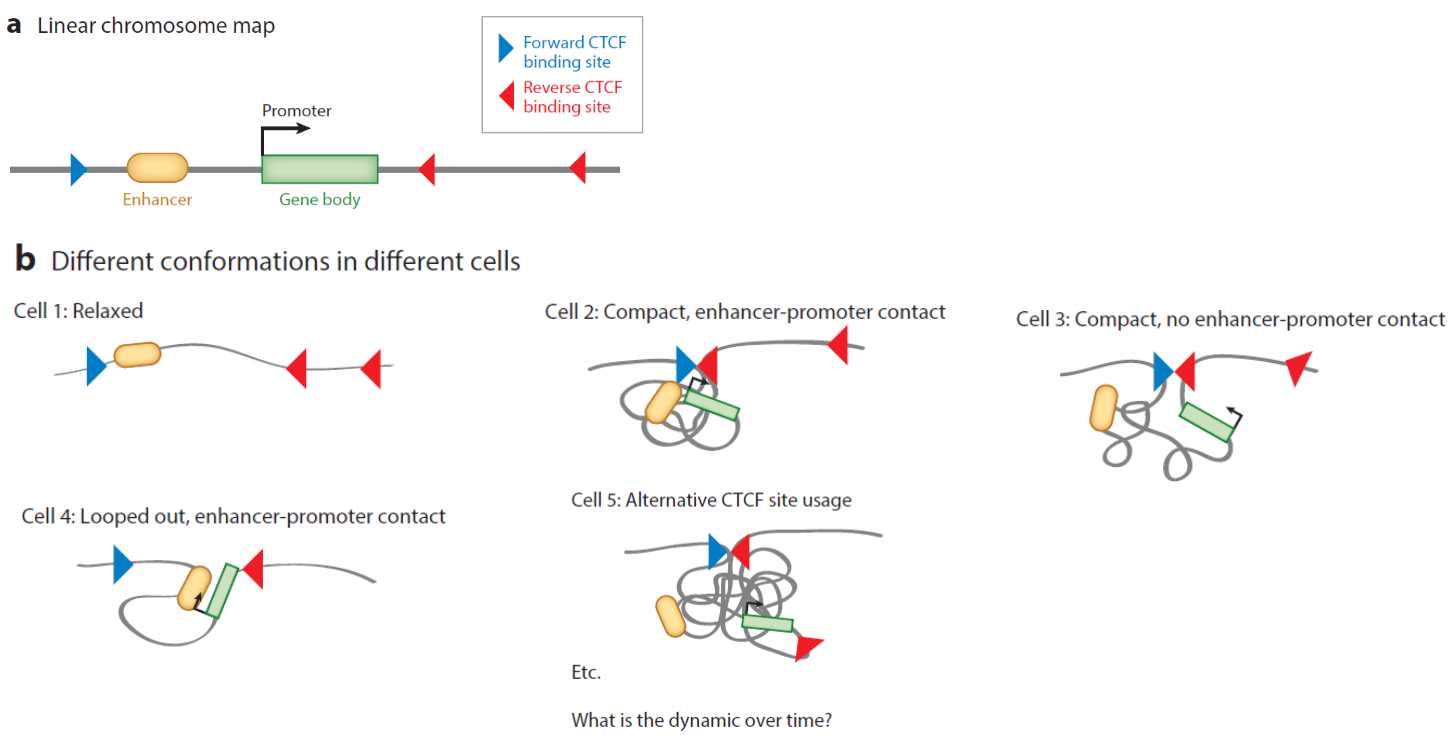
\includegraphics[width=0.8\textwidth]{../_resources/Screenshot_2022-10-19_at_08-48-41.png}
\caption{Merkenschlager and Nora, Ann Rev Gen Hum Genetics, 2016}
\end{figure}

\hypertarget{chromosome-conformation-capture-3c}{%
\section{Chromosome Conformation Capture (3C)}\label{chromosome-conformation-capture-3c}}

This method is used to verify whether distant sequences are interacting in their 3D folding. 3D conformations at the regional, chromosome and whole genome levels can be inferred by calculating the number of ligation junctions between genomic loci.

It is required to have information on all sequences of interest. It is possible to apply inverse PCR: we circularize and amplify from known primers a piece of unknown sequence. In order to test a bigger region, we can use specific primers and verify which sequence is mapped where (computational analysis).

ChIA-PET: which protein is mediating the interaction among two sequences? Use antibody for the protein of interest e.g.~CTCF, pull down cross linked, digest and sequence.

Lastly, in Hi-C approach there is a fill in of the extremities of the restriction sites with biotin and direct sequencing $\rightarrow$ higher throughput.

\hypertarget{hi-c-approach}{%
\section{Hi-C approach}\label{hi-c-approach}}

\begin{enumerate}
\def\labelenumi{\arabic{enumi}.}
\tightlist
\item
  HindIII restriction enzyme
\item
  Fill extremities and mark with biotin
\item
  Ligate (Nhel)
\item
  Purify and shear DNA; pull down biotin
\item
  Sequence using paired-end
\end{enumerate}

A Hi-C map, or \textbf{contact matrix}, is a list of DNA-DNA contacts produced by a Hi-C experiment. Spatial proximity maps of the human genome generated with Hi-C at a resolution of 1 megabase. Each pixel represents all interactions between a 1-Mb locus and another 1-Mb locus.

\begin{figure}
\centering
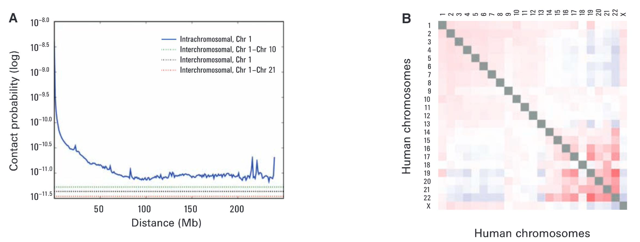
\includegraphics[width=0.7\textwidth]{../_resources/Screenshot_2022-10-25_at_11-47-30.png}
\caption{Lieberma-Aiden \emph{et al., Science} 2009}
\label{fig:int}
\end{figure}

By changing the restriction enzyme, a similar pattern is observed. The closer two sequences are in linear form, the higher their contact probability (frequency of interaction).

The probability of contact decreases as a function of genomic distance on chromosome 1. Interchromosomal interactions are depleted relative to intrachromosomal interactions. The level of interchromosomal contact differs for different pairs of chromosomes. This suggests that the chromosomes form defined territories, with an overall frequency of interaction (Figure \ref{fig:int}).

Depending on the chromosome, we can find preferential contacts. Example: 20-21-22 region. In low resolution, we observe conserved interaction for synthetic or orthologous sequences.

Each chromosome can be decomposed into two sets of loci (arbitrarily labeled A and B) such that contacts within each set are enriched and contacts between sets are depleted. Regions tend be closer in space if they belong to the same compartment (A versus B). Bimodal pattern in eigenvector $\rightarrow$ either A or B compartment.

Figure \ref{fig:fish}: 3D-FISH to probe four loci (L1, L2, L3, and L4) on chromosome 14 that alternate between the two compartments (L1 and L3 in compartment A; L2 and L4 in compartment B).

\begin{figure}
\centering
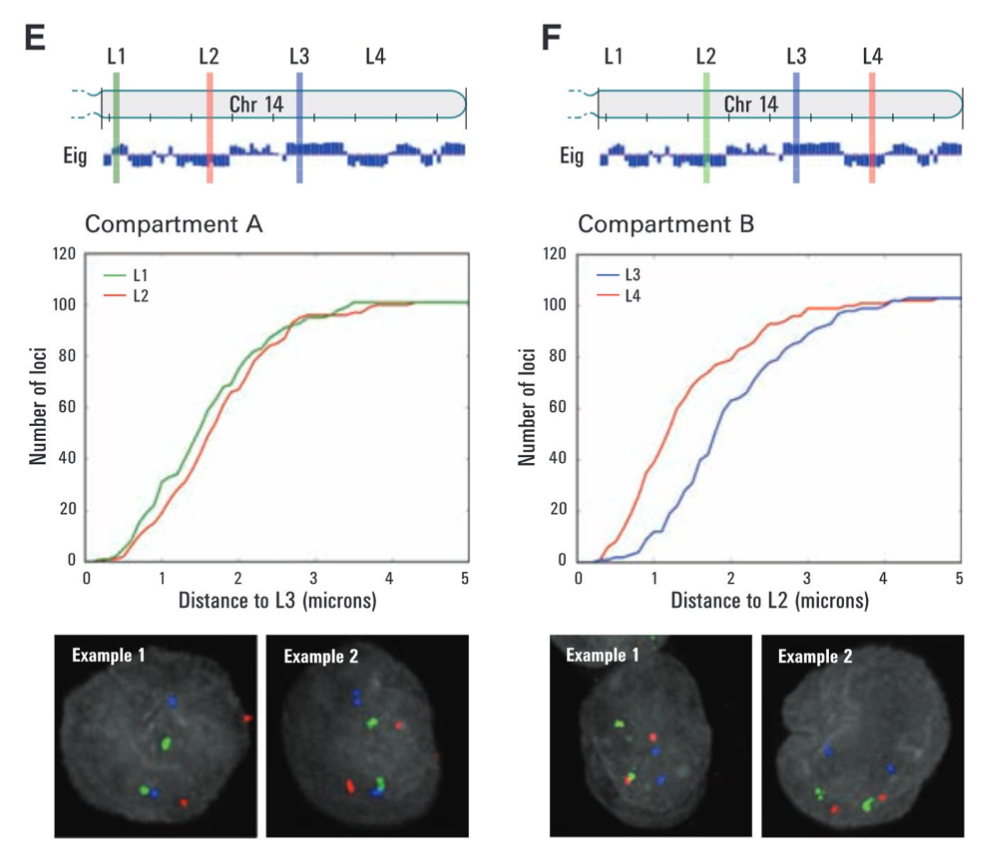
\includegraphics[width=0.5\textwidth]{../_resources/Screenshot_2022-10-19_at_09-06-00.png}
\caption{Lieberma-Aiden \emph{et al., Science} 2009}
\label{fig:fish}
\end{figure}

\begin{itemize}
\tightlist
\item
  Compartment B showed a consistently higher interaction frequency at a given genomic distance than pairs of loci in compartment A, suggesting that it is more densely packed.
\item
  Compartment A correlates strongly with the presence of genes, higher mRNA expression, and accessible chromatin, as measured by DNAse I sensitivity.
\item
  Open and closed chromatin occupies different compartments in the nucleus.
\item
  Such partitioning of the human genome was obtained based on the contact frequency of millions of loci at 1 Mb resolution.
\end{itemize}

\hypertarget{optimization-of-hi-c-approach}{%
\subsection{Optimization of Hi-C approach}\label{optimization-of-hi-c-approach}}

Digestion \emph{in situ}, permeabilize nuclei from cells and - without lysing them -  introduce a restriction enzyme cutting 4 nucleotide bases $\rightarrow$ 1kb resolution (Figure \ref{fig:kb}), proximity ligation performed in intact nuclei reducing the frequency of spurious contacts).

\begin{figure}[!htb]
   \begin{minipage}{0.48\textwidth}
     \centering
     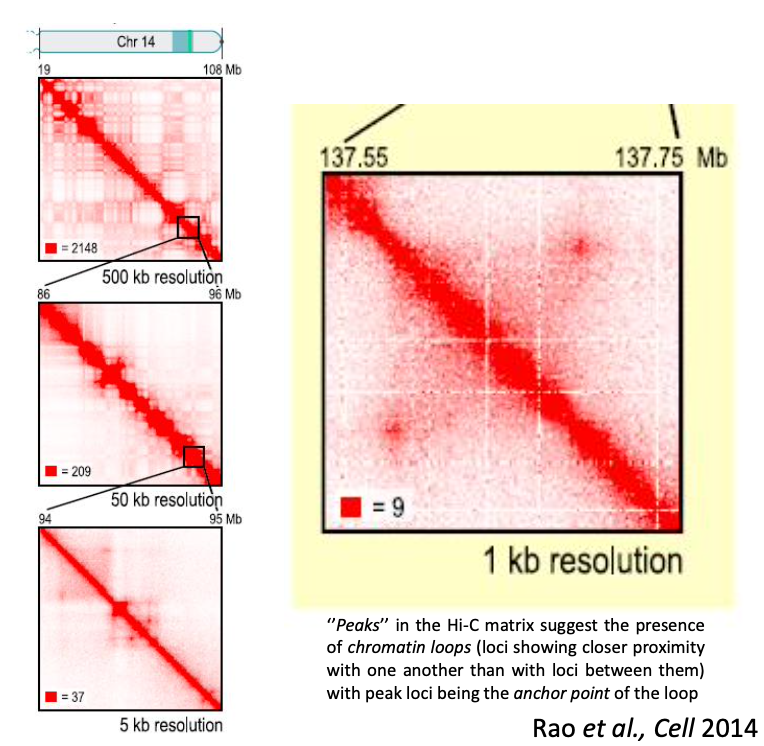
\includegraphics[width=0.7\linewidth]{../_resources/Screenshot_2022-10-19_at_09-10-50.png}
     \caption{}\label{fig:kb}
   \end{minipage}\hfill
   \begin{minipage}{0.48\textwidth}
     \centering
     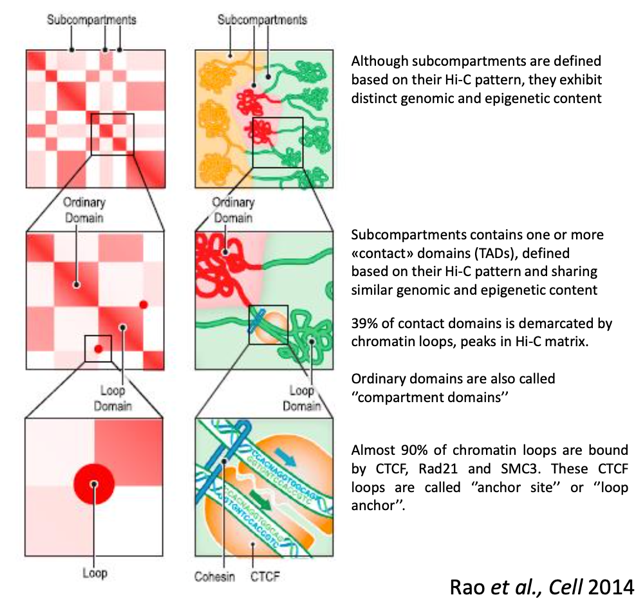
\includegraphics[width=0.7\linewidth]{../_resources/Screenshot_2022-10-19_at_09-11-30.png}
     \caption{}\label{fig:sub}
   \end{minipage}
\end{figure}

We can divide a compartment in 6 subcompartments: A1,A2,B1,B2,B3 and B4. The genomic and epigenetic content is different: different density of active genes, CG richness, epigenetic marks,\ldots{} If we increase the resolution within subcompartments, we find frequently interacting regions, which are called domains (Figure \ref{fig:sub}):

\begin{itemize}
\tightlist
\item
  \emph{loop domains} (90\% bound by TFs, they are also called ``anchor sites'')
\item
  \emph{ordinary domains or compartment domains}
\end{itemize}

Chromosome compartments are formed by the aggregation of multiple domains with similar biochemical or functional properties. In literature some studies indicate ``sub-TADs'' or ``insulated neighborhoods'' to refer to domains identified by high-resolution Hi-C as being smaller than the domains TADs, either ordinary or loop domains.

The frequency of interaction can also be depicted as a linear genomic coordinate. A Hi-C map can be integrated with ChIP-seq and RNA-seq data to assess the complexity of the domains identified by low resolution data.

The identification of TADs is highly dependent on the resolution of the Hi-C data and the scale at which the data are analysed.

\begin{figure}
\centering
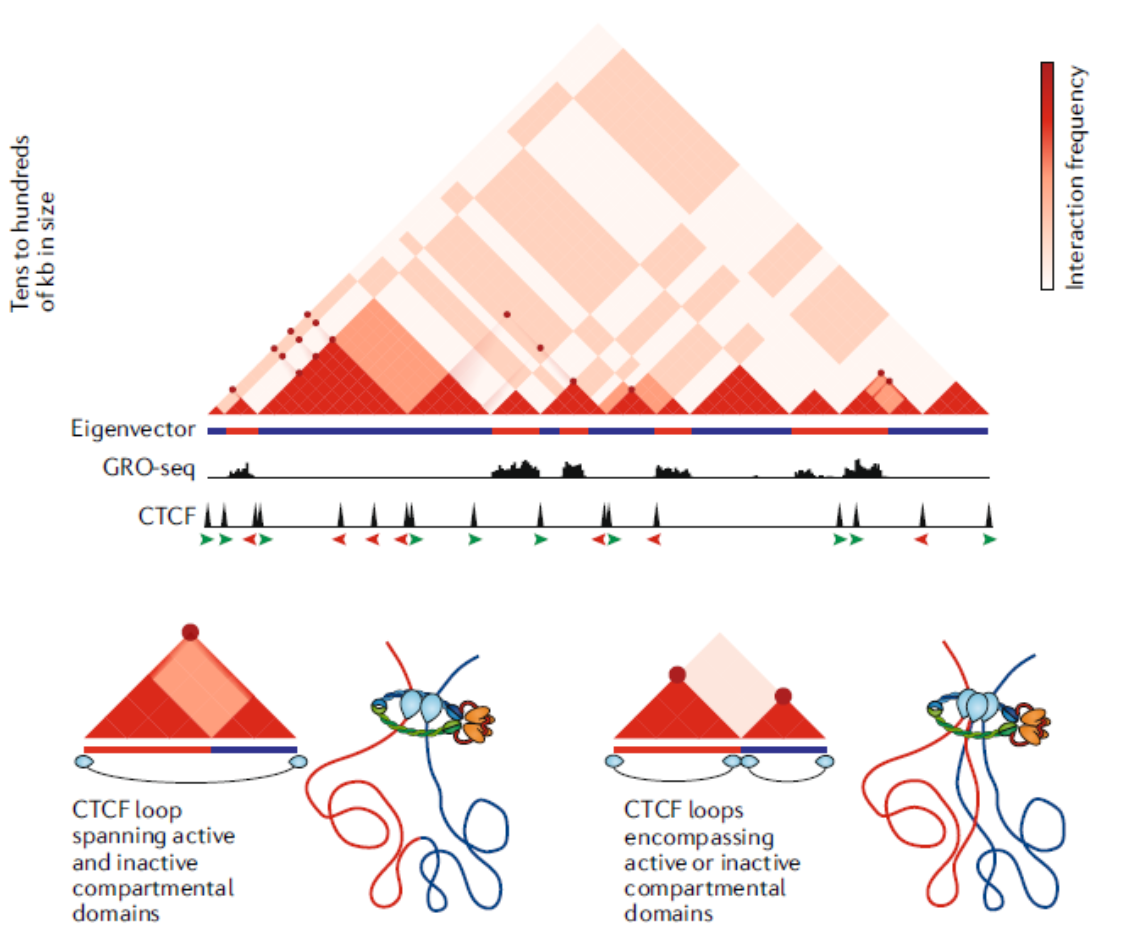
\includegraphics[width=0.5\textwidth]{../_resources/Screenshot_2022-10-19_at_09-20-57.png}
\caption{Rowley and Corces, \emph{Nature Rev Genetics} 2018}
\end{figure}

Some CTCF loops encompass active and inactive domains.

\begin{figure}
\centering
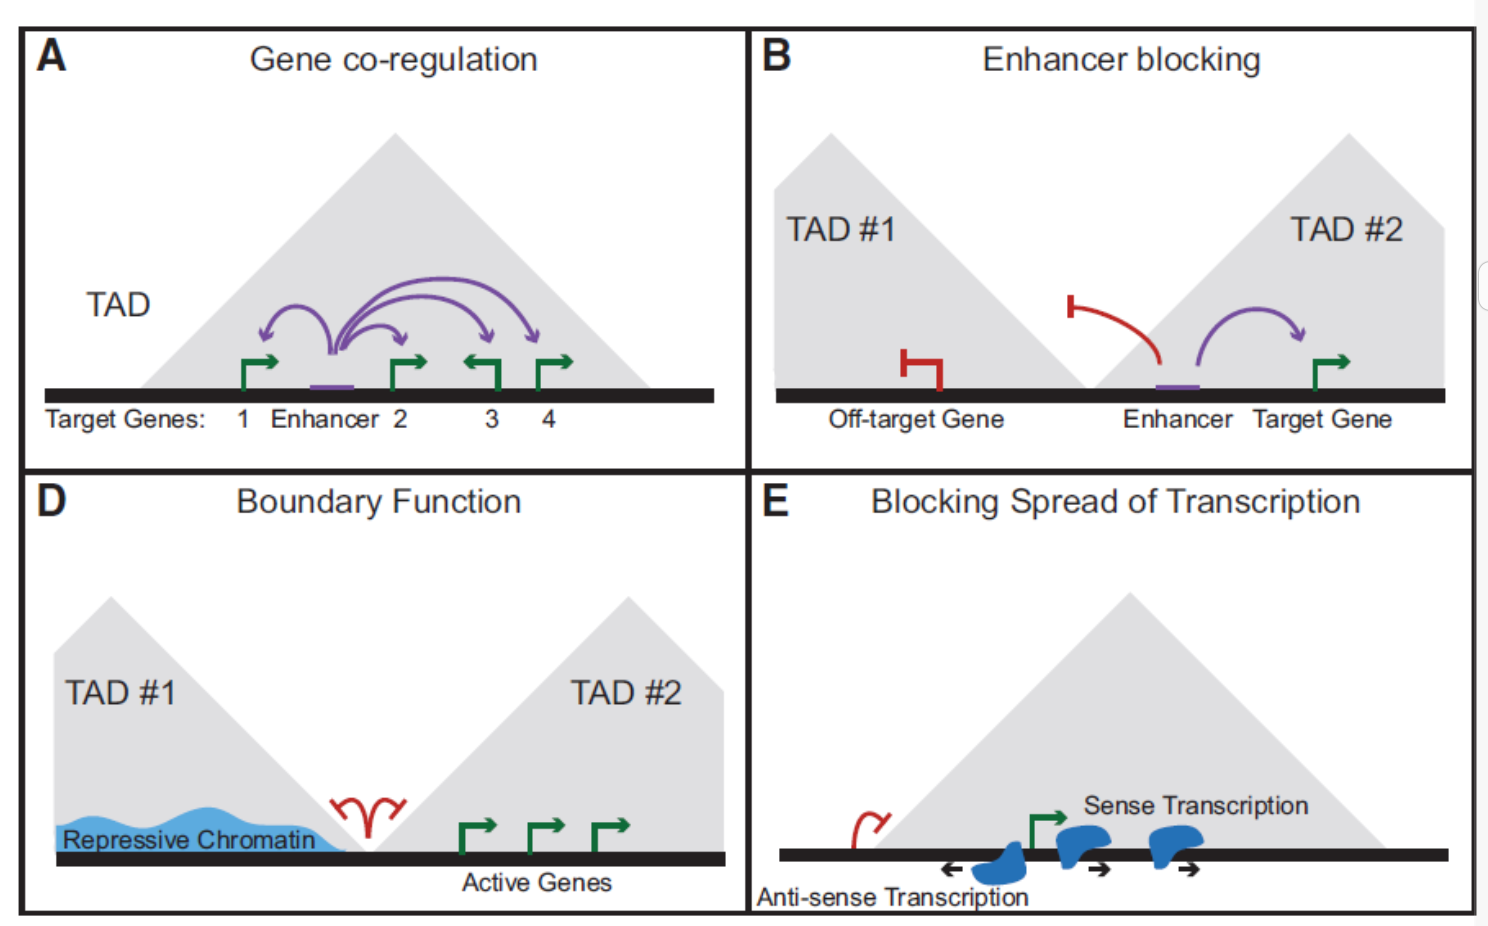
\includegraphics[width=0.5\textwidth]{../_resources/Screenshot_2022-10-19_at_09-21-57.png}
\caption{Dixon \emph{et al., Mol Cell.} 2016}
\end{figure}

Given the high frequency of interaction, we can observe co-regulation favouring. Also, since different TADs do not contain frequently interacting genes, a TAD could feature enhancer blocking. Boundary function: ability of repressing the spreading of heterochromatin. 

\textbf{Conclusions:}

\begin{itemize}
\tightlist
\item
  Genomes are partitioned into `contact domains' (ordinary domains or loop domains), or TADs, with median length of 185 kb, that share similar chromatin states and tend to associate with each other forming subcompartments (some people refer TADs to the subcompartments)
\item
  CTCF and the cohesin associate with loop domains and are found at over 86\% of loop anchors
\item
  The pair of CTCF motifs present at the loop anchors occurs in a convergent orientation in \textgreater90\% of cases
\item
  Loops frequently link promoters and enhancers, correlate with gene activation, and show conservation across cell types and species (up to 75\% are conserved between cell lines, and 50\% between mouse and human orthologous genomic regions)
\end{itemize}

\section{Mediator and cohesin connect gene expression and chromatin architecture}

Enhancers and genes generally interact within the context of the CTCF-CTCF loops, which form insulated neighborhoods that constrain interactions between regulatory elements and genes.
This structure helps explain why enhancers generally control only a limited number of genes despite having an ability to function in either orientation and at long distances.

Do enhancers and promoters randomly interact within the same loop domain? Probably not, since single CTCF loops can contain both active and inactive genes. Enhancer-gene interactions occur in insulated neighborhoods by the synergistic activity of Mediator and Cohesin, and not CTCF.

Mediator and cohesin physically and functionally connect the enhancers and core promoters of active genes within DNA loop domains in murine embryonic stem cells. When the transcription activators bind the mediator, the mediator complex undergoes a conformational change, and this activator-bound form of mediator binds cohesin and its loading factor Nipbl, which all contribute to gene activity and DNA looping. Mediator and cohesin co-occupy different promoters in different cells, thus generating cell-type-specific DNA loops linked to the gene expression program of each cell.

There are different binding sites for cohesin mediator and cohesin CTCF. We observe distinct overlapping pattern in interaction sites, depletion by shRNA results in a very similar gene expression.

\textbf{Co-IP:}

\begin{enumerate}
\def\labelenumi{\arabic{enumi}.}
\tightlist
\item
  lysate and wash
\item
  add antibody-immobilized agarose resin
\item
  precipitate immune complexes and wash
\item
  analysis by Western blot (nuclear extract vs Co-IP with IgG control)
\end{enumerate}

Adapt Co-IP with ChIP: protein in chromatin complex, instead of extracting RNA de-crosslink and run protein on a gel.

Co-IP results indicate that Cohesin and Mediator interact. Chromosome Comformation Capture (3C) analyses confirmed DNA looping between promoters and enhancers of active genes. Depleting cohesin, frequency of interaction is disrupted, similar as Mediator 12.

\hypertarget{promoter-enhancer-communication-occurs-primarily-within-insulated-neighbourhoods}{%
\subsection{Promoter-Enhancer Communication Occurs Primarily within Insulated neighbourhoods}\label{promoter-enhancer-communication-occurs-primarily-within-insulated-neighbourhoods}}

Computational analyses of published CTCF and Smc1 ChIA-PET datasets enabled the identification of insulated neighborhoods encompassing 9,407 protein-coding genes of which 3,929 were transcriptionally active in mouse ESCs (Figure \ref{fig:mouse}).

\begin{figure}
\centering
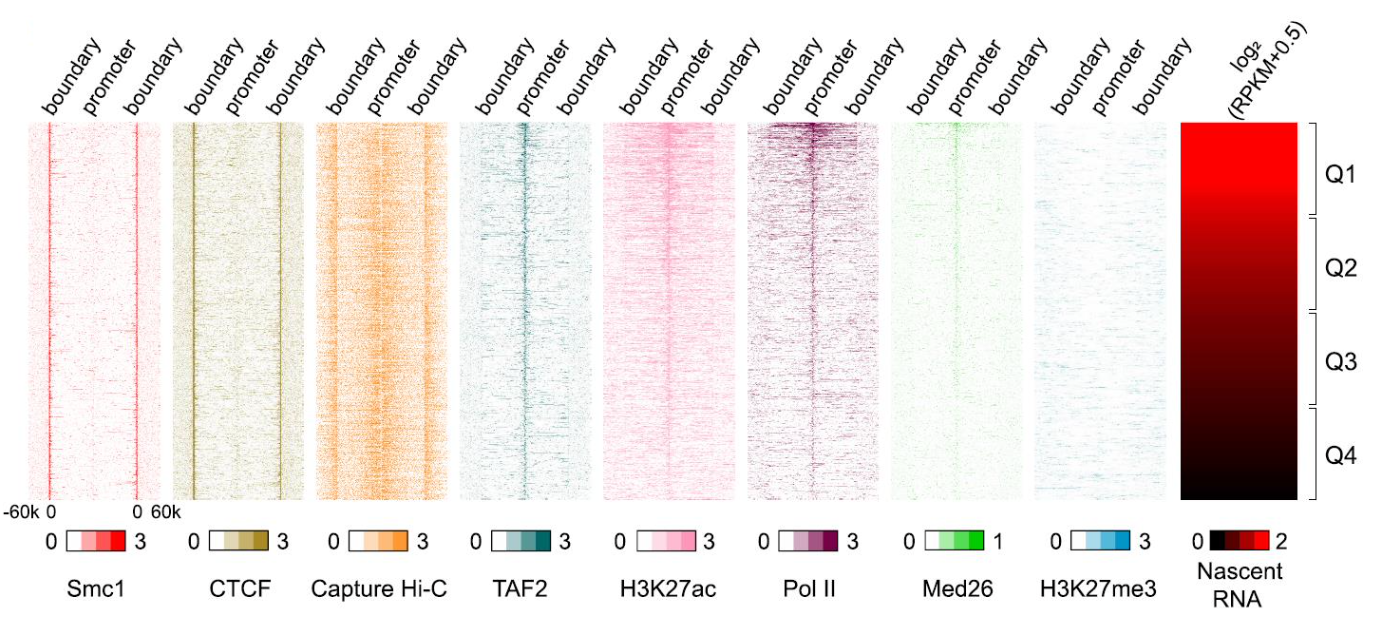
\includegraphics[width=0.5\textwidth]{../_resources/Screenshot_2022-10-19_at_10-01-09.png}
\caption{Sun et al., 2019}
\label{fig:mouse}
\end{figure}

The sites of co-binding of cohesin and CTCF define \emph{DNA loops boundaries}. We can recognize promoters by TAF2 Hac, POL II (not much Med26, repressive).

The main enrichment is at the boundaries, its functional meaning has not yet been defined. We can group promoters in quartiles (Q1-Q4) according to efficiency of transcription. The extent of interaction in loops is not necessarily dependent on the frequency of interaction. Capture Hi-C showed that almost 80\% of promoter-interacting loci are constrained within the insulator or at the boundaries; these interactions do not correlate with transcription levels. 

Can the Mediator complex be removed from specific genes? A sequence with promoter and TF binding site was generated and anchored to a magnetic bead.  The binding of the protein was tested with a Western blot. The transcription factor estrogen-related receptor b (\textbf{Essrb}) directly interacts with the Mediator complex. Downregulating Essrb would impair Mediator binding to specific enhancers, deregulating expression of distinct target genes. Indeed, Essrb knock down can be used to deplete Mediator, inactivate enhancers and downregulate target genes.

Now that a system to inactivate enhancers is in place, the authors can test whether enhancer function is constrained within insulated neighborhoods. 222 insulated neighborhoods contained genes downregulated more than 2 folds upon Essrb depletion. Transcription regulation is largely constrained within insulated neighborhoods, and it involves TF-mediator interactions. \emph{Is this regulation directly related to promoter- enhancer looping?}

\subsection{Depletion of Mediator causes loss of PIC assembly}

Most enhancer-promoter interactions occur in DNA loops, also called insulated neighborhoods. 
Hypothesis: oncogenes are present in DNA loops, which can be activate by different mechanisms, listed in Figure \ref{fig:proto}.

\begin{figure}
\centering
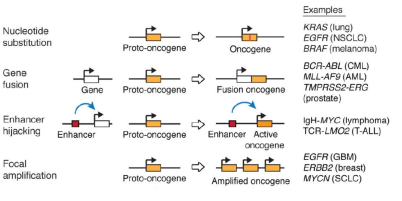
\includegraphics[width=0.5\textwidth]{../_resources/4eb79fba5a169cc3d31f5400dee44c80.png}
\caption{Hnisz et al., Cell, 2016}
\label{fig:proto}
\end{figure}

\emph{Is there a way for DNA loops to promote oncogene transcription?}

In Jurkat cells , 9038 CTCF loops were identified with median length of 270 kb, containing 2-3 genes on average. They crossed adult and embryonic cell lines to discover TADs. Through other analyses they found out that most cohesin associated enhancer-promoter interactions occur within CTCF-CTCF loops.

40/55 known oncogenes in the cell line map in insulated neighborhoods. E.g: LMO2 would not usually be transcribed because enclosed in the loop, but with the help of super-enhancers, proto oncogenes like TAL1 can be transcribed.

\textbf{Both active oncogenes and silent proto-oncogenes are located within insulated neighborhoods in Jurkat cells}. 
The main hypothesis states that some insulated neighborhoods function to prevent proto-oncogene activation, then some T-ALL tumor cells may have genetic alterations that perturb the CTCF bourdaries of neighborhoods containing T-ALL oncogenes.

Example: deletion in promoter of TAL1 $\rightarrow$ its transcription is initiated by STIL promoter, which is normally active in T-Cells. TAL1 is usually silenced after fetal stage. Using CRISPr/Cas9 they removed a little piece on the boundary. Disruption of insulated neighborhood boundaries is linked to proto-oncogene activation (Figure \ref{fig:cas}).

The silent state of the TAL1 proto-oncogene is dependent on the integrity of the insulated neighborhood. TAL1 encodes a transcription factor that is overexpressed in \textasciitilde50\% of T-ALL cases and is a key oncogenic driver of this cancer (Figure \ref{fig:tal1}).

\begin{figure}[!htb]
   \begin{minipage}{0.48\textwidth}
     \centering
    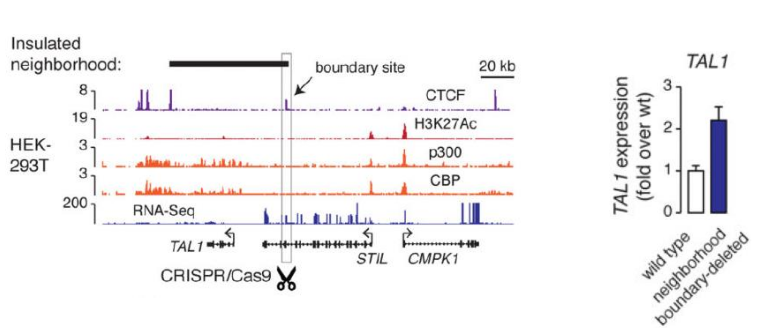
\includegraphics[width=0.5\textwidth]{../_resources/bf32b9679af0fb7fcba57b9f87bb4207.png}
\caption{Hnisz et al., Cell, 2016}
\label{fig:cas}
   \end{minipage}\hfill
   \begin{minipage}{0.48\textwidth}
     \centering
    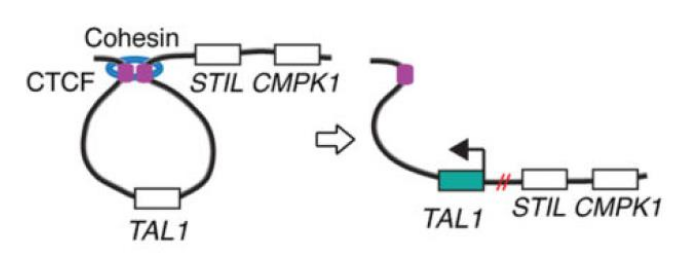
\includegraphics[width=0.5\textwidth]{../_resources/3d83d920d425aa5f76bdbb127596c02b.png}
\caption{Hnisz et al., Cell, 2016}\label{fig:tal1}
   \end{minipage}
\end{figure}

They tried to do the same on another locus, without the mediation of enhancers or promoters. Even in this case,  the disruption of DNA loop allows for the transcription of proto oncogenes.

CTCF in constitutive neighborhoods (present in all cell lines) has a somatic mutation in this cancer, but not the ones in non-boundary CTCF sites (specific to the cell lines). It becomes clear that somatic mutations of insulated neighborhood boundaries occur in the genomes of many different cancers.

\textbf{Main conclusions of the article:}
\begin{itemize}
\item Disruption of insulated neighborhood boundaries, marked by the presence of CTCF and cohesins,
can cause oncogene activation in cancer cells
\item Recurrent perturbations of boundary elements may impact expression of genes with roles in
tumor biology
\end{itemize}

\hypertarget{super-enhancers}{%
\section{Super-enhancers}\label{super-enhancers}}

Super-enhancers regulate genes involved in cell identity: they are bound by tissue-specific TFs and pioneer transcription factors such as OCT4, SOX2, NANOG. They generally activate a self-regulatory circuit: most SE produce promoters, which in turn regulate their own SE and other gene products that they lead.

TAL1 forms transcriptional regulatory networks with other transcription factors in hematopoietic stem cells (Figure \ref{fig:hema}).

\begin{figure}[!htb]
   \begin{minipage}{0.48\textwidth}
     \centering
     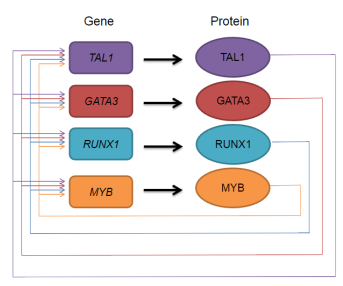
\includegraphics[width=0.3\textwidth]{../_resources/99fbd93b812d482263d53c442698a36a.png}
\caption{}
\label{fig:hema}
   \end{minipage}\hfill
   \begin{minipage}{0.48\textwidth}
     \centering
     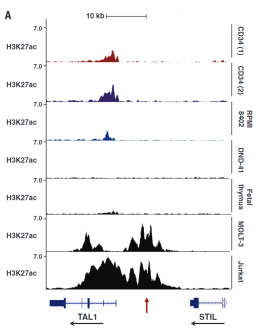
\includegraphics[width=0.3\textwidth]{../_resources/c099d4a9ad4bba13e7839f48fd831265.png}
\caption{}
\label{fig:talju}
   \end{minipage}
\end{figure}

These circuits underline the tissue-specificity of most cancers. TAL1 requires a SE, a transcriptional re-wiring.
\begin{itemize}
\item The expression of TAL1 is downregulated during normal T-cell development, while GATA3 and RUNX1 are expressed in T cells
\item  Re-expression of TAL1 in T cells dictates a transcriptional circuitry inducing tumorigenesis
\item TAL1, GATA3, RUNX1 and MYB gene loci are associated with super-enhancers in T-ALL cells
\end{itemize}

\hypertarget{how-is-a-se-generated-during-tumorigenesis}{%
\subsection{How is a SE generated during tumorigenesis?}\label{how-is-a-se-generated-during-tumorigenesis}}

Even SNPs can generate super-enhancers. TAL1 SE was not found in T cells, or hematopoietic stem and progenitor cells (HSPCs). 3C experiments identified a looping interaction within the SE (red arrow), not anymore an insulated neighborhood in this particular site (Figure \ref{fig:talju}).

While investigating the reason for this difference, they found out some nucleotide addition (but not much). A small insertion leads to a TFBS in T-ALL cancer cell lines. Only transcription factors expressed in T-ALL cells are involved in the activation of the mutant enhancer.

But a mutation in the promoter of TAL1 is not enough. We need all the transcription circuit of the actors that co-regulate each-other. The Mediator binding pattern stretching for 20kb, overlapping with the H2K27ac mark (seen in previous ChIP), indicates the presence of a super-enhancer. Not observed in HPSCs or T-ALL cells devoid of the mutated TAL1 enhancer site: it is the de novo MYB site to promote TAL1 complex formation and induce TAL1 expression.

ChIP seq revealed the presence of a TAL1 complex, including MYB, at the TAL1 mutated enhancer.
Targeted deletion of the TAL1 enhancer mutation collapses the TAL1 super-enhancer (Figure \ref{fig:deltal}). This results in a gain of function even in heterozygosity. A SE can be generated by a single transcription factor biding site and can extend to hundred of bases. They are very sensitive to mutations.

Finally, there's mainly two ways to activate proto-oncogenes (Figure \ref{fig:sup}). Both can be triggered by very short deletions/mutations that happen in regulatory regions.

\begin{figure}[!htb]
   \begin{minipage}{0.48\textwidth}
     \centering
    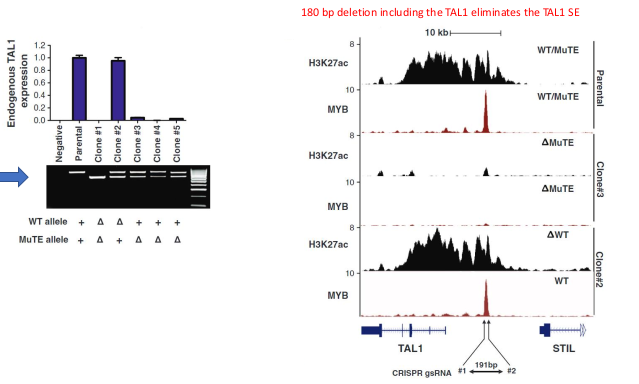
\includegraphics[width=0.7\textwidth]{../_resources/dfb8371fc17e078308c3d5aa247ebcbf.png}
\caption{}
\label{fig:deltal}
   \end{minipage}\hfill
   \begin{minipage}{0.48\textwidth}
     \centering
     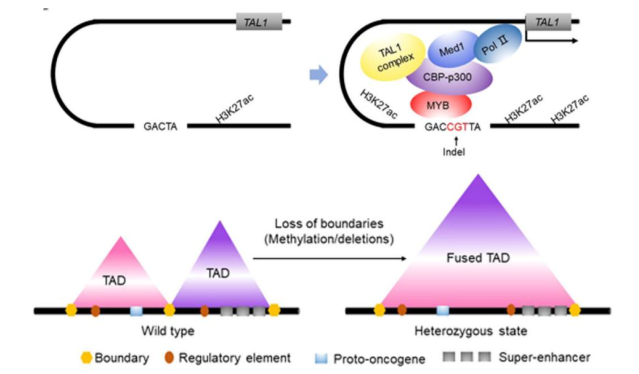
\includegraphics[width=0.7\textwidth]{../_resources/8bd5f4820c364c35b02c35eb0e48f464.png}
\caption{}
\label{fig:sup}
   \end{minipage}
\end{figure}

More recent genomic insertions form enhancers that misregulate oncogenes; this hypothesis was tested in different cancer cell lines.

\hypertarget{how-cancer-cells-take-advantage-of-super-enhancers}{%
\subsection{How cancer cells take advantage of super-enhancers}\label{how-cancer-cells-take-advantage-of-super-enhancers}}

In the study \textbf{Identification of focally amplified lineage-specific super-enhancers in human epithelial cancers}, scientists interrogated a dataset of 10k tumors and found recurrent focal amplifications, with 25 peaks corresponding to super-enhancers. They also found that six different cancer cell types had some common recurrent focal amplification in the same spot (Figure \ref{fig:study}).

\begin{figure}
\centering
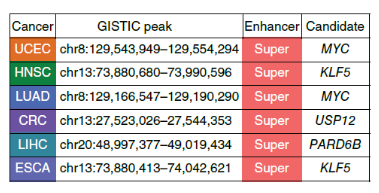
\includegraphics[width=0.5\textwidth]{../_resources/796c982294bedb0a7994a942aa5ff2a5.png}
\caption{}
\label{fig:study}
\end{figure}

\begin{itemize}
\item UCEC, uterine corpus endometrial carcinoma; 
\item HNSC, head and neck squamous cell carcinoma; 
\item LUAD, lung adenocarcinoma; 
\item CRC, colorectal carcinoma; 
\item LIHC, liver hepatocellular carcinoma; 
\item CESC, cervical squamous cell carcinoma; 
\item ESCA, esophageal carcinoma.
\end{itemize}

For MYC genes, they found data in two different cancer lines. Selectivity of amplification depends on the cell line.
Tumors with amplification of MYC alone or MYC-LASE or MYC-ECSE alone express higher levels of MYC than tumors lacking either amplification (meaning, there's no need for the tumor to evolve a over-expression of MYC).

NFE2L2 and CEBPB transcription factors regulate the e3 enhancer; to study it, we can downregulate these two factors.

\textbf{Conclusion: MYC regulation changes based on the tumor and tissue type.}
If we are in a cancer setting, we can target a super-enhancer and we impact the expression of the target gene. However, there are several onco-genes in a cancer setting.

\hypertarget{the-role-of-myc-in-cancer-cells}{%
\section{The role of MYC in cancer cells}\label{the-role-of-myc-in-cancer-cells}}

In cancer, MYC is always the most amplified gene. MYC is the downstream target of many pro-proliferation pathways and has a huge effect on cells.

\begin{figure}
\centering
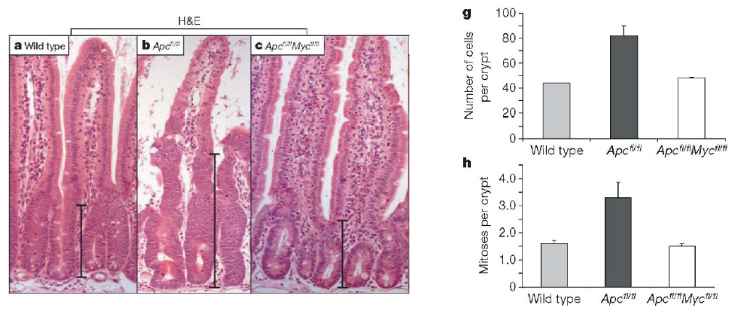
\includegraphics[width=0.5\textwidth]{../_resources/641af477cb65d73954e1ae24aab9a2ed.png}
\caption{Deletion of both Myc and APC from small intenstine cells}
\label{fig:inhi}
\end{figure}

The inhibition of MYC and APC rescues or prevents tumorigenesis. By removing one single target gene, we can have drastic results and MYC is capable of driving tumorigenesis on its own (Figure \ref{fig:inhi}).

In most human tumour types, the expression of MYC proteins is deregulated and enhanced relative to the corresponding normal tissue, and high MYC expression often correlates with poor prognosis. \textbf{MYC induces cell proliferation and growth} in the absence of external growth factors. Conversely, inhibition of MYC almost invariably suppresses cell proliferation.
Transgenic mouse studies provided the evidence that deregulated expression of MYC is sufficient to drive tumorigenesis in a number of transgenic mouse tissue.

\hypertarget{key-aspect-of-myc-in-tumorigenesis}{%
\subsection{Key aspects of MYC in tumorigenesis}\label{key-aspect-of-myc-in-tumorigenesis}}

\begin{figure}
\centering
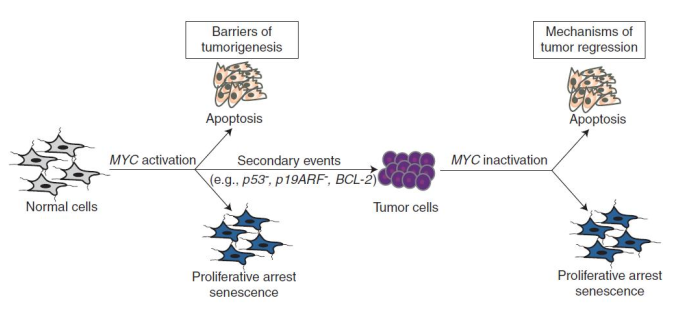
\includegraphics[width=0.5\textwidth]{../_resources/18345a0e70ca9e50883ca61f93ad3405.png}
\caption{Gabai et al., CSHL 2014}
\label{fig:key}
\end{figure}

Cells become addicted to a single oncogene (and to transcription in general). The key aspects of MYC are recapitulated in Figure \ref{fig:key}.

\hypertarget{myc-transcription-factor-forms-a-heterodimer-with-max}{%
\subsubsection{MYC transcription factor forms a heterodimer with MAX}\label{myc-transcription-factor-forms-a-heterodimer-with-max}}

MYC is quite an unstable protein, even its mRNA has a very short life. It has an one-of-a-kind binding domain, it is a very special protein.

\begin{figure}
\centering
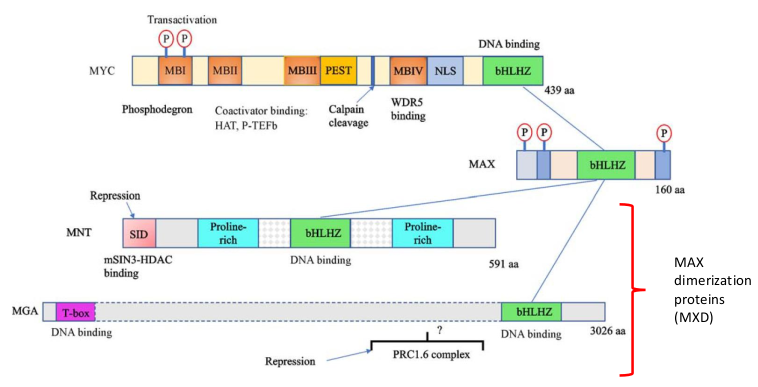
\includegraphics[width=0.5\textwidth]{../_resources/01adbb32a69ee3baec1bf9bddd890f52.png}
\caption{ MYC is a transcription factor forming a heterodimer with MAX}
\label{fig:myc}
\end{figure}

MYC, MAX and MXDI all recognise the same binding site (Figure \ref{fig:myc}).
MXD and MYC act as antagonists. MXD proteins can recruit histone deacetylases and repress transcription while MYC proteins recruit complexes that promote transcription (not always the case\ldots). MYC stimulates cell growth and proliferation, while MXD inhibits cell growth and proliferation and blocks MYC effects.
MYC-MAX bind to thousands of genes whose identity depends on the cellular transcriptome and the abundance of MYC protein (Figure \ref{fig:maxmyc}).

Studying MYC is very difficult. What we know is that if we do a chIP for MYC we have an extreme range of possible results, i.e, result is basically random. For RNA-seq: regulation of genes from MYC is also very subtle, with down-up regualted genes changing like 20\%, but also transcribe for TF that regulate their own site.

\begin{figure}[!htb]
   \begin{minipage}{0.48\textwidth}
     \centering
    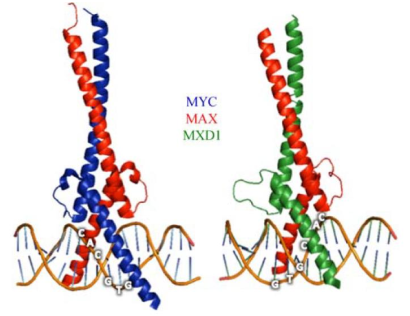
\includegraphics[width=0.5\textwidth]{../_resources/017e543a7782177edd93188be60ae382.png}
	\caption{Carroll et al., Front.Med. 2018}
	\label{fig:maxmyc}
   \end{minipage}\hfill
   \begin{minipage}{0.48\textwidth}
     \centering
     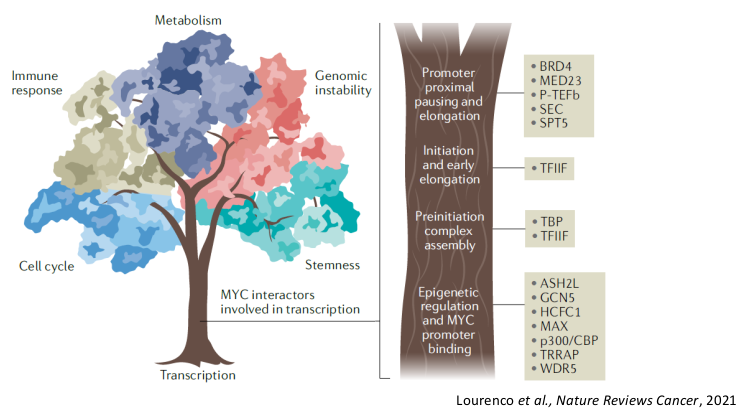
\includegraphics[width=0.7\textwidth]{../_resources/e218faf59750ef1a90a9e45629f08973.png}
	\caption{Lourenco et al., Nature Reviews Cancer, 2021}
	\label{fig:regmyc}
   \end{minipage}
\end{figure}

\begin{figure}
\centering
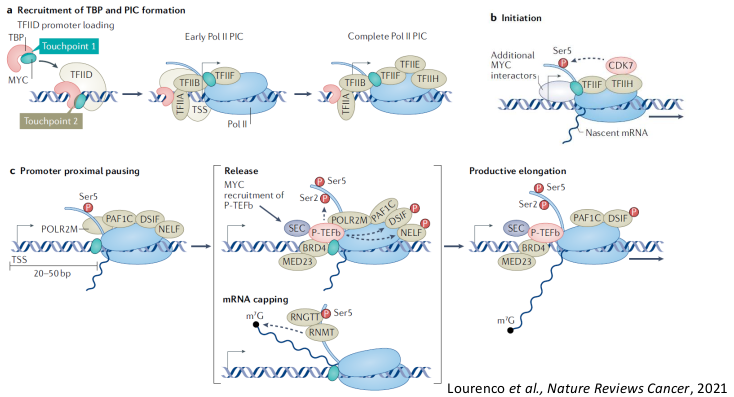
\includegraphics[width=0.7\textwidth]{../_resources/10a2ad3114504053030a1071443aabd7.png}
\caption{Lourenco et al., Nature Reviews Cancer, 2021}
\label{fig:ppmyc}
\end{figure}

MYC is not a pioneer TF, hence the interaction with proteins recruited on chromatin is highly relevant.
With open chromatin state, we have un-specific transcription. In addition to the regulation of its own target genes, MYC can `\textbf{amplify}' the transcriptional program already active in a cell, leading to a signature which is cell type-specific. MYC increases the expression of (already poised) thousands of genes (Figure \ref{fig:ppmyc}). It depends a lot on the level of MYC2: since there are low affinity and high affinity binding sites, the more the MYC, the higher the probability of MYC binding the low-affinity regions.  However, tumorigenesis is not only about proliferation: we need proteins, membranes,\ldots{} obviously MYC is also involved in anti-apoptosis behaviour, energy metabolism etc.

\begin{figure}
\centering
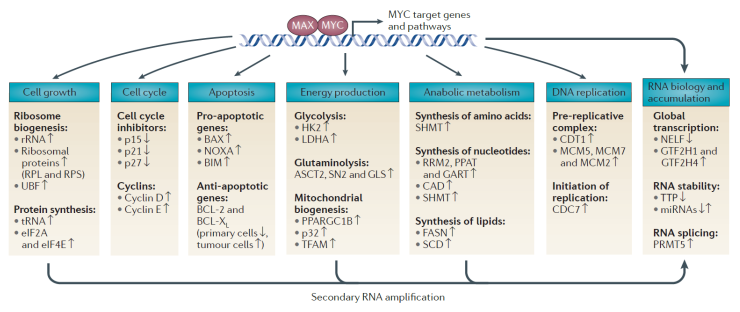
\includegraphics[width=0.7\textwidth]{../_resources/cdb9692b7dd2ca7bcfae696cd1b1ce36.png}
\caption{Kress et al, NatureRevCancer-2015}
\label{fig:ppmyc}
\end{figure}

\hypertarget{by-which-major-mechanism-or-pathway-myc-proteins-promote-tumorigenesis}{%
\subsection{By which major mechanism or pathway do MYC proteins promote tumorigenesis?}\label{by-which-major-mechanism-or-pathway-myc-proteins-promote-tumorigenesis}}

The final outcome of MYC gene regulation depends on the network of MYC interactions, in particular MYC-MAX
and MAX-MXD, and by the transcriptional program of the cells.
MYC is a mild transcriptional modulator, inducing moderate changes in mRNA levels.
It is able to regulate the expression of several other transcription factors and cofactors, including E2F proteins,
Polycomb group repressive complex 2 (PRC2) components, along with microRNAs (miRNAs), thus orchestrating
complex networks of gene regulation.
MYC dependent gene regulation has been shown to be dependent on: cell type, experimental conditions (stress),
levels of MYC.

In conclusion, MYC activation contributes to several hallmarks of cancer:
\begin{enumerate}
\item autonomous proliferation and growth
\item sustained DNA replication
\item increased protein biogenesis
\item global changes in cellular metabolism
\item activation of the angiogenic switch
\item suppression of the response to autocrine and paracrine regulatory programs
\item restraint of host immune responses
\item the transcription rewiring induced by oncogenic Myc levels also renders cancer cells addicted to this particular oncogene
\end{enumerate}
